\papersection{Implementing the \libos{}}


The \libos{} of \graphene{}, or 
\thelibos{},
is a single library that resides beneath a Linux application,
for exporting compatible Linux features and API.
\thelibos{} guarantees reuse of an unmodified Linux application
upon \thehostabi{},
regardless of host limitations or distinctions.
%upon an incompatible host OS or hardware.
%to support compatible OS features.
%for exporting compatible features.
An unmodified Linux application assumes the existence of a Linux kernel or equivalent,
with OS-specific features and characteristics,
or {\bf Linux personality}.
%which an unmodified Linux application depends on.
%In order to reuse an unmodified Linux application
%on an incompatible host,
\thelibos{} reproduces the Linux personality,
to act as a guest-level Linux kernel.
%over various host options.
%using \thehostabi{} exported by the host OS and PAL.
%The purpose of \thelibos{}
%is to resue an unmodified Linux application,
%by combining with a PAL and a host OS to behave as an equivalence of a Linux kernel. 
%%which is developed upon the assumption of running on a Linux kernel or equivalent.
%The main purpose of \thelibos{} is to reproduce
%the idiosyncratic features and behaviors of Linux,
%or the {\bf Linux personality},
%to resurrect Linux applications upon incompatible
%host OSes or hardware.
\graphene{} develops \thelibos{} as an ELF dynamic library (i.e., \code{\tt libLinux.so}),
and the PAL dynamically loads \thelibos{}.
%to be loaded on a host by the corresponding PAL.
%at the beginning of a \picoproc{}.


A key component of \thelibos{}
is a Linux system call table, which redirects system calls from a Linux application.
%a key Linux kernel component applications. 
%that \thelibos{} implements is the Linux system call table.
%For Linux and similar OSes,
A system call table is an important entry point to a Linux kernel.
A system call table contains
pointers to the kernel functions for each system call,
indexed by the system call numbers (e.g., \code{NR\_open} or 10 on x86-64).
%and triggers in-kernel operations for servicing requests from applications.
%and defines the interaction between applications and kernel.
\graphene{} moves the Linux system call table into \thelibos{},
and develops system call handlers in the user space.
%The system call table in \thelibos{} contains a number of system call handlers,
Each system call handler emulates
the semantics of a system call,
% that \graphene{} supports;
%\graphene{} develops each handler
based on either the specification % known by the Linux application developers,
described in the man pages~\cite{linux-man-syscall},
or the bug-for-bug behaviors
observed in a real Linux kernel.
Some system calls, such as \syscall{rt\_sigaction}, are partially documented
in the man pages, and \thelibos{} imitates a Linux kernel on implementing a poorly-documented system calls.
%\graphene{} grows the \thelibos{} functionality
%by extending the guest-level Linux system call table
%with more complete implementation.

%Otherwise, for a few system calls whose behaviors
%are not clearly defined by the Linux manpages,
%such as \syscall{rt\_sigaction},
%the system call handlers mimic the bug-for-bug behaviors of an actual Linux kernel.
%A continuing goal in \graphene{} is
%to extend \thelibos{} with more complete system call handlers.


%grow the functionality of \thelibos{},
%by extending the system call table with more complete handlers.




%The development of system call handlers in \thelibos{}
%is equivalent to implementing the specifications described in the Linux man pages~\cite{linux-man-syscall},
%including the valid inputs to each system call,
%as well as the expected outcome.


%\paragraph{Implementing Linux Personality.} 
%\fixmedp{Revisit the logical flow of these paragraphs}
\Thelibos{} currently implements \graphenesyscallnum{} system calls,
and is sufficient to run a range of applications from servers to command-line programs or runtimes.
For reference, a recent Linux kernel supports more than 300 system calls.
A Linux kernel also
contains a long tail of infrequently-used system calls.
%upon \thehostabi{}. % to interact with the host.
%Among the whole Linux system call table,
%A Linux kernel exports a long tail of infrequently-used system calls.
%For reference, the Linux \linuxversion{} kernel exports \linuxsyscallnum{} system calls.
A study of the Linux system call usage~\cite{tsai16apistudy}
indicates that only 40 system calls are indispensable to every applications released in the Ubuntu official repositories.
%The study also shows that
In the meantime, more than 100 system calls are used by only exactly one application,
or none at all.
The development of \thelibos{} began with
implementing 12 system calls, such as \syscall{read} and \syscall{open}, which are fundamental to running a ``hello world'' application,
%such as \syscall{read}, \syscall{write}, and \syscall{open},
and gradually grows the system call count.
%for each new application introduced to run on \graphene{}.
%As the count of system calls continues to grow,
Each time \thelibos{} is tested against a new application, the number of system calls that need to be added has dropped.
%Based on the types of applications priorized in \graphene{}, including servers, command-line programs, and language runtimes, some system calls to be more important %for reusing the applications
%than the others. % system calls.
%According to the usage of each system call in applications,
\graphene{} prioritizes the popular system calls, and leaves other system calls that are either unpopular or for administrative purposes such as rebooting
or configuring network interfaces.
\thelibos{} demonstrates the sufficiency of
implementing Linux system calls upon \thehostabi{},
for a representative subset of applications, .


%The current \thelibos{} implementation
%includes a set of high-valued Linux system calls for the types of applications
%that \graphene{} has targeted,
%including servers, command-line programs, and runtimes.
%The remaning system calls may require extending \thehostabi{} with more privileged abstractions,
%including administrative operations
%and host-specific features.
%\thelibos{} demonstrates that \thehostabi{} is sufficient
%for exporting the host abstractions, to support a representative sample of Linux applications.

%such as memory sharing, scheduler configuration, and NUMA (non-uniform memory architecture) support.


%Linux exports a very long tail of infrequently-used system calls.
%applications.




%An analysis indicates roughly 100 additional calls that can be implemented
%with the existing \pal{} ABI and coordination framework, less than 10 administrative calls that will not make sense to expose to 
%an application, such as loading a kernel module or rebooting the system, and roughly 54 that will require 
%\pal{} extensions to meaningfully implement, such as controlling scheduling,
%NUMA placement, I/O privilege, and shared memory.
%In the last category of system calls, the degree to which actual host details should be exported versus emulated is debatable.

%We believe represent the most commonly used system calls.
%When an application requests a call or argument that {\tt libLinux.so} does not implement,
%the picoprocess exits with a distinct error message. 
%Each time we have tested \graphene{} with a new application, the number of extra system calls
%required has dropped---most recently we only added 4 calls
%(namely, epoll\_create, epoll\_wait, semget and semop)
%to support the Apache web server.
%Thus, we believe \graphene{} implements a representative sample of Linux calls.

%such as {\tt sched\_setparam}, which manipulates scheduler-specific
%parameters or 
%{\tt uselib}, which has been abandoned 
%in {\tt glibc} version 2 in favor of a user-space dynamic linker.
%We do not plan to implement administrative interfaces, such as {\tt reboot}.
%The growth in the set of supported system calls has been driven by 
%the requirements of new applications we use to exercise \graphene{}, and has been 
%slowing considerably over time.



\papersubsection{System call redirection}
\label{sec:libos:syscall-redirection}


\thelibos{} transparently redirects system calls from a Linux application. In a Linux kernel, a system call interrupt handler
triggers the kernel operations
whenever an application executes
a ``\assembly{syscall}'' or ``\assembly{int \$80}'' instruction.
The interrupt handler
switches the context of application,
and then jumps to the kernel routines which serve the system calls.
%based on a kernel convention agreed by applications and Linux kernels.
Because \thelibos{} reuses
unmodified Linux executables and libraries,
it must redirect
unmodified system call invocation
to its
system call table. % implemented inside \thelibos{}.
%intercepts the system calls
%in an executable or library binary, and redirect the system calls
%to the system call handlers inside \thelibos{}.
%\thelibos{} implements the callback functions for a subset of the Linux system calls.
%For reference, Linux kernel \linuxversion{}
%has defined \linuxsyscallnum{} system calls in total.


Normally,
\thelibos{} redirects system calls %from an unmodified Linux application
by modifying the C library (\libc{}).
%from an unmodified Linux application.
Most Linux executables and libraries
are linked against \libc{},
and rely \libc{} functions to access OS features
instead of
invoking system calls directly.
%but use \libc{} functions as wrappers to system calls.
%which internally execute ``\code{syscall}'' or ``\code{int \$80}'' instructions.
%an executable or library in Linux and similar OSes invokes system calls through \libc{},
%instead of directly containing the \code{syscall} instructions.
%The \libc{}
%contains a large set of system call wrappers,
%which encapsulate direct system calls to the kernel as functions.
For example,
compared with making the \syscall{read} system call directly,
more commonly
an application uses \libc{}'s \code{stdio} functions,
or calls the \libc{} \syscall{read} wrapper
%\funcname{read} is a wrapper to,
which internally runs \assembly{syscall}.
% that bares the same name and definition.
Unless configured otherwise, \thelibos{} uses a modified
{\bf GNU C library (\glibc{})}~\cite{glibc},
as the standard GNU \libc{} of most Linux distributions, including Ubuntu.
%applications released by Ubuntu. % are compatible against \glibc{}.
%which is compatible against most of the Linux applications released for Ubuntu.
%Other \libc{} variants, ,
%which are either fully or partially compatible with \glibc{},
%can be also modified to redirect system calls to \thelibos{}.
%are alternatives upon \thelibos{} as long as they are modified for .
\graphene{} can be configured to use other \libc{} variants,
such as \projname{uClibc}~\cite{uclibc} and \projname{musl}~\cite{musl},
if an application finds them sufficient.
%\graphene{} demonstrates that 
%are also demonstrated
%to be acceptable alternatives,
%with slight modification for system call redirection.




\graphene{} modifies only \gipclines{} lines of the \glibc{} code.
\glibc{} uses a platform-independent macro,
%referenced a single macro called
\funcname{INLINE\_SYSCALL},
to invoke system calls.
%when it needs to invoke a system call.
The macro \funcname{INLINE\_SYSCALL} contains assembly code
that copies system call number and arguments to registers,
and then uses \assembly{syscall} to enter a Linux kernel.
\graphene{} modifies \funcname{INLINE\_SYSCALL}
to redirect a system call to
an entry point of \thelibos{} called \funcname{syscalldb}.
\funcname{syscalldb} saves the current register state, similar to a context switch,
and then
calls the system call handler
indicated by the system call number.
%, to trigger operations inside \thelibos{}.
For assembly code in \glibc{},
\graphene{} replaces each \code{syscall} instruction with
a dynamic call to
\funcname{syscalldb}, given the address of \funcname{syscalldb} is dynamically determined.
Figure~\ref{fig:libos:syscall-redirection} summarizes the mechanism of system call redirection.
%to \thelibos{}.


\begin{figure}[t!]
\centering
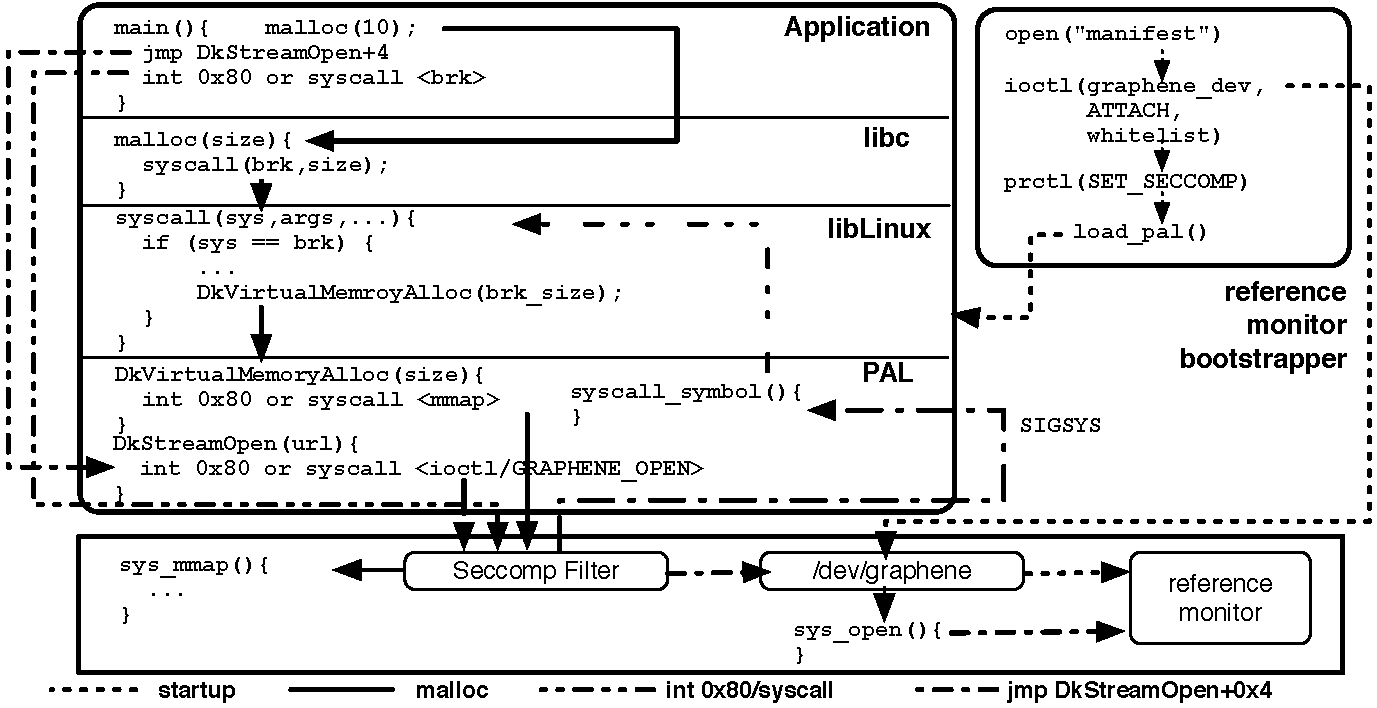
\includegraphics[width=32em]{syscall-redirection.pdf}
\footnotesize
\caption{System call redirection for \thelibos{}.
In the normal case (the first instruction of \funcname{main}), \funcname{malloc} internally invokes 
\syscall{mmap}, which is redirected to \funcname{syscalldb} in \thelibos{}.\thelibos{} then invokes a \hostapi{}, \palcall{VirtMemAlloc}, to allocate host memory. The second instruction of \funcname{main} invokes a direct system call, which is trapped by the host-level exception handler,
and returned to \funcname{IllegalInstrHandler} in \thelibos{}.}
\label{fig:libos:syscall-redirection}
\end{figure}


\graphene{} modifies four \glibc{} libraries:
%When using \graphene{}, an application must be deployed with the modified \libc{} libraries,
a runtime dynamic loader (\code{ld.so}), a core library (\code{libc.so}), a POSIX thread library (\libpthread{}), and a dynamic loading library (\libdl{}).
Each of the \Glibc{} libraries has separate purposes and features,
and is mostly loaded on demand except \code{ld.so}.
%Despite that \glibc{} has partitioned its code into separate libraries,
\graphene{} only modifies the \glibc{} libraries which contains direct \assembly{syscall} instructions.
%not every libraries of \glibc{} need to be modified for system call redirection.
%Only \code{libc.so}, \libpthread{}, and \libdl{} have included \code{syscall} instructions,
%and thus have to be modified for \graphene{}.
Other libraries, such as \code{libm.so},
only rely on 
existing \libc{} functions,
so \graphene{} leaves these libraries unmodified.



\paragraph{Hard-coded system calls.}
Static binaries, or some platform-dependent applications, contain hard-coded \assembly{syscall} instructions
which cannot be redirected by a modified \libc{}.
Application developers
create a static binary with with hard-coded system calls by statically linking a local version of \libc{} as part of the binary.
%as a static binary with hard-coded system calls. %\code{syscall} instructions.
It is also possible to program an application
with assembly code that directly invokes system calls---usually in a language runtime (e.g., the go runtime) or a system software (e.g., \projname{busybox}).
%---with assembly code that directly invokes
%platform-depenedent,
%rare system calls that are not wrapped by \libc{} functions.
%one of the system call wrappers in \libc{}, or \funcname{syscall}.
%As a result, a ELF binary may contain hard-coded \assembly{syscall} instructions.
%Either way leads to hard-coding \code{syscall} instructions in the ELF binaries.
Because a modified \libc{} cannot redirect hard-coded system calls,
the application switches context into the host kernel,
causing security and compatibility breaches by exposing unauthorized or unsynchronized host OS states to the application.



\thelibos{} needs support from a host OS to restrict direct system calls from an application.
%\thelibos{} depends on host-level system call restriction to redirect hard-coded system calls.
%to prevent system calls from anywhere other than a PAL.
A Linux kernel allows an application to install a system call filter in the Berkeley Packet Filter (BPF) format,
called a \seccomp{} filter~\cite{seccomp}.
A \seccomp{} filter can block or forward a system call based on the system call number,
argument values, or the code address that invokes the system call.
%A direct system call traps into the host kernel,
%unless the host has virtualized the interrupt handler to the \libos{}.
\graphene{} relies on the hosts to install a system call filter, or enforce architectural restriction, to detect direct system calls.
For example, \sgx{} already has a restriction that an enclave application cannot trigger any system call to switch context into the untrusted kernel.
% inside an enclave and triggers an exception for an in-enclave system call.
%\code{syscall} instructions
%(e.g., \sgx{} restriction).
%The details of the system call restriction mechanisms are discussed in
%\fixme{update labels}
%Section~\ref{sec:linux:syscall} and Section~\ref{sec:sgx:syscall}.
If the host detects a direct system call from an application,
it can return
a PAL exception to an exception handlers assigned by \thelibos{}, using  \palcall{ExceptionSetHandler}.
%\thehostabi{} specifies that the host captures unauthorizes system calls
%and redirects to an exception handler (set up by \palcall{ExceptionSetHandler}).
%If a binary makes an illegal system call,
%the host-level system call restriction will trigger an \code{ILLEGAL} exception
%at \thehostabi{},
%and thus the system call is redirected by an exception handler
%assigned by \thelibos{}.
The exception handler can recover the system call number and arguments
from the context saved at the system call,
and forward the system call to the system call handler
inside \thelibos{}.


Using exceptions to forward direct system call is much slower than redirecting through a modified \libc{},
due to the overhead of switching context between the application and the host kernel.
To handle an exception from the host OS,
the application at least switches context twice, including both triggering the exception handler and returning to the original execution.
To mitigate the overhead,
\thelibos{} can 
rewrite the hard-coded \assembly{syscall} or \assembly{int \$80} inside each application binary during the run time.
% to redirect the hard-coded system calls;
%use {\bf binary translation} to modify the hard-coded \code{syscall} instructions;
There can be two timings for rewriting the instructions:
One is the timing when the runtime loader a new binary, and \thelibos{} can perform a full scan of the binary
to replace \assembly{syscall} or \assembly{int \$80} with a jump to \thelibos{}'s system call table.
\thelibos{} can also passively replace the instructions
whenever the host detects a direct system call and triggers an exception handler.
%binary translation
%can be triggered when a host-level exception is raised
%for an illegal system call,
%to optimize consecutive system call invocation at the same location.
%\thelibos{} can also perform a full scan in application binaries
%to spot and modify hard-code \code{syscall} instructions.
\graphene{} leaves binary rewriting
as a future feature.


